% =====================================================================
%  DeepScan – Zweistufige ML-Pipeline (TikZ)
%  ---------------------------------------------------------------------
%  Eigenständig kompilierbar (standalone). Zum Einbinden in die Arbeit
%  den tikzpicture-Block in eine figure-Umgebung kopieren. Pakete:
%  \usepackage{tikz}\usetikzlibrary{positioning,arrows.meta,shapes.geometric,fit,backgrounds}
% =====================================================================
\documentclass[border=8pt]{standalone}
\usepackage{tikz}
\usepackage[scaled]{helvet}\renewcommand\familydefault{\sfdefault}
\usetikzlibrary{positioning,arrows.meta,shapes.geometric,fit,backgrounds,calc,shadows}

\begin{document}
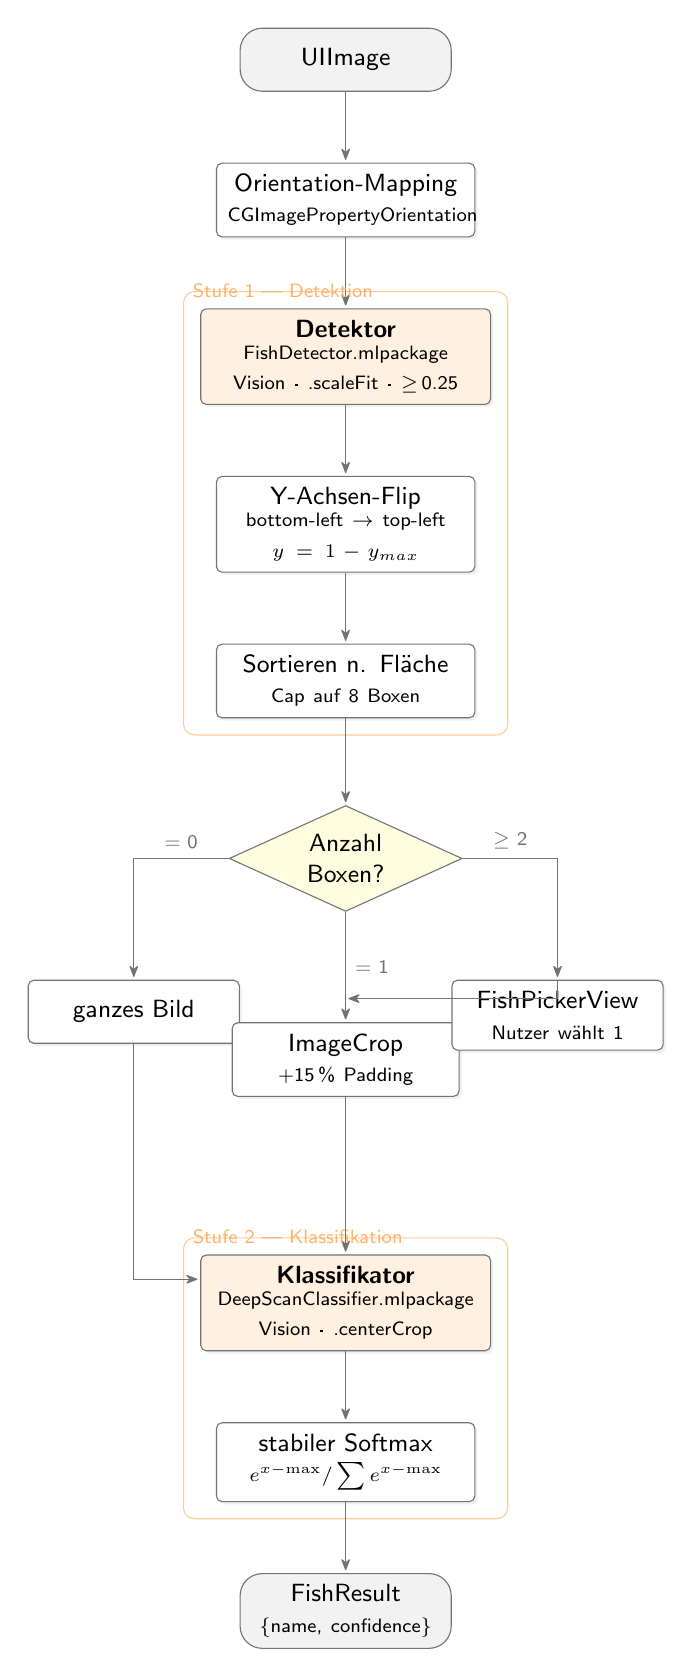
\begin{tikzpicture}[
    font=\small,
    >={Stealth[round]},
    node distance=9mm,
    io/.style={draw=black!55, rounded corners=8pt, fill=black!5, align=center,
               minimum height=8mm, inner sep=4pt, text width=24mm},
    proc/.style={draw=black!55, rounded corners=2pt, fill=white, align=center,
                 minimum height=8mm, inner sep=4pt, text width=30mm,
                 drop shadow={opacity=0.12,shadow xshift=1pt,shadow yshift=-1pt}},
    model/.style={proc, fill=orange!12, text width=34mm},
    dec/.style={draw=black!55, fill=yellow!12, diamond, aspect=2.2, align=center,
                inner sep=1pt, text width=14mm},
    flow/.style={->, draw=black!55, shorten >=1pt},
    lbl/.style={font=\scriptsize, text=black!55},
]

% ---- Input + preprocessing ----------------------------------------
\node[io] (img) {UIImage};
\node[proc, below=of img] (orient) {Orientation-Mapping\\\scriptsize CGImagePropertyOrientation};

% ---- Stage 1: Detector --------------------------------------------
\node[model, below=of orient] (det) {\textbf{Detektor}\\\scriptsize FishDetector.mlpackage\\\scriptsize Vision · .scaleFit · $\geq$\,0.25};
\node[proc, below=of det] (yflip) {Y-Achsen-Flip\\\scriptsize bottom-left $\to$ top-left\\\scriptsize $y = 1 - y_{max}$};
\node[proc, below=of yflip] (sortc) {Sortieren n. Fläche\\\scriptsize Cap auf 8 Boxen};

% ---- Decision -----------------------------------------------------
\node[dec, below=11mm of sortc] (cnt) {Anzahl Boxen?};

% ---- Three branches -----------------------------------------------
\node[proc, below left=12mm and 6mm of cnt, text width=24mm] (whole) {ganzes Bild};
\node[proc, below=14mm of cnt, text width=26mm] (crop1) {ImageCrop\\\scriptsize +15\,\% Padding};
\node[proc, below right=12mm and 6mm of cnt, text width=24mm] (pick) {FishPickerView\\\scriptsize Nutzer wählt 1};

% ---- Stage 2: Classifier ------------------------------------------
\node[model, below=20mm of crop1] (cls) {\textbf{Klassifikator}\\\scriptsize DeepScanClassifier.mlpackage\\\scriptsize Vision · .centerCrop};
\node[proc, below=of cls] (soft) {stabiler Softmax\\\scriptsize $e^{x-\max} / \sum e^{x-\max}$};
\node[io, below=of soft] (res) {FishResult\\\scriptsize \{name, confidence\}};

% ---- Edges --------------------------------------------------------
\draw[flow] (img) -- (orient);
\draw[flow] (orient) -- (det);
\draw[flow] (det) -- (yflip);
\draw[flow] (yflip) -- (sortc);
\draw[flow] (sortc) -- (cnt);

\draw[flow] (cnt) -| (whole) node[pos=0.25,above,lbl]{= 0};
\draw[flow] (cnt) -- (crop1) node[pos=0.5,right,lbl]{= 1};
\draw[flow] (cnt) -| (pick)  node[pos=0.25,above,lbl]{$\geq$ 2};
\draw[flow] (pick) |- ($(crop1.north)+(0,3mm)$);

\draw[flow] (whole) |- ($(cls.west)+(0,3mm)$);
\draw[flow] (crop1) -- (cls);
\draw[flow] (cls) -- (soft);
\draw[flow] (soft) -- (res);

% ---- Stage frames -------------------------------------------------
\begin{scope}[on background layer]
    \node[draw=orange!40, rounded corners=4pt, inner sep=6pt, fit=(det)(yflip)(sortc)] (S1) {};
    \node[draw=orange!40, rounded corners=4pt, inner sep=6pt, fit=(cls)(soft)] (S2) {};
\end{scope}
\node[lbl, anchor=west, text=orange!60] at (S1.north west) {Stufe 1 — Detektion};
\node[lbl, anchor=west, text=orange!60] at (S2.north west) {Stufe 2 — Klassifikation};

\end{tikzpicture}
\end{document}
